\chapter{Project Evaluation}

% evaluate the product, and see whether we have at least the minimum viable product
% using the requirements and design goals (possibly in a table)
% make sure to add lots and lots of figures, tables and benchmarks here
% also add SIG stuff and talk about SCRUM

\todo{Put results in appendix F}
\todo{write conclusion about results}

\section{Validation and Verification}
In this subsection, we first describe how the system is tested and how we measure the quality of the code with SIG \cite{sig}. Afterwards we define a protocol with which the results of the system can be evaluated for correctness. We will first evaluate the results of the classification, and afterwards the relation scores. These are related in the sense that a relation score is calculated by the number of occurrences in labelled documents, so the correctness of labelling affects the correctness of relation scores. The results can be found in section \ref{app:val_ver_results}.\\

\subsection{Testing the Application}
We will test the program using four different testing methods. The first is unit testing, which tests the separate components individually. Next comes integration testing, to see how well different components work together. Afterwards we use system testing for testing the different system components. Lastly, acceptance testing is used for testing how well the clients think the program works.

\subsubsection{Unit Tests}
Unit testing is done by writing automatic tests and making sure they pass every time the tests are executed. Unit tests test each method of a function separately, checking that the method does what it is supposed to do. If the method would need information from outside the class that information is mocked. This means that instead of using that other class, a fake object is made which returns a fake value. This ensures the tests will never fail due to changes in other classes.

\subsubsection{Integration Tests}
Integration testing uses automated tests which test how well different components of the system work together. This is done more or less the same as unit testing, however whilst you would mock methods from other classes in unit testing, with integration testing you do not. It is assumed that the separate modules are unit tested, therefor if an error occurs it is because something is wrong with the interaction between the modules and not with the modules themselves. 

\subsubsection{System Tests}
We are also planning to use system testing. System testing provides a more complete test of the entire system. This means it is useful to detect faults in the overall system, but less easy to determine where these faults may be located. System testing is done manually, which means the tests can not be easily repeated when the system changes whilst with other testing techniques this is possible.

\subsubsection{Acceptance Tests}
Last we use acceptance testing. This is testing done to see if the software does what the clients are expecting it to do. These tests are therefore also executed by the clients manually. Afterwards they can say what worked, what did not work, what was missing and what could be improved. For this, we set up an evaluation protocol.

\subsection{SIG}
SIG \cite{sig}, short for software improvement development group, is an organisation that analyses the code of projects to give insights in the quality of how the code is written. A high score means the code is highly maintainable and is kept simple. SIG includes Better Code Hub \cite{better_code_hub} which checks our code according to 10 guidelines as can be seen in appendix \ref{bch_guidelines}. The great thing about Better Code Hub is that it can be run at anytime. We can check Better Code Hub whenever, whilst for SIG we have to send in our code and wait for feedback. 

\subsection{Evaluating the Classification}
There are several ways to evaluate machine learning algorithms. We will base our evaluation of the classifier on the guidelines of the Microsoft Azure Machine Learning evaluation model \cite{EvualteML}. According to the page binary classification can be evaluated with the following metrics: Accuracy, Precision, Recall, F1 and AUC.

\subsubsection{Accuracy}
Accuracy is the proportion of correctly classified instances. This however a poor indication of how well the classifier works. For instance if you have a test set of 100 websites, of which 90\% belongs to Category A. Than if the classifier simply predicts all websites to belong to category A the accuracy would be 90\%. It would seem the classifier performs well, but it actually fails to classify the other 10\% of the websites correctly.

\subsubsection{Confusion Matrix}
A page can only either belong to class A (positive), or not belong to class A (negative). If a page is predicted by the classifier correctly it is called true positive (TP) or true negative (TN). If the classifier predicts the page incorrectly it results in a false positive (FP) or false negative (FN). This can be seen in the confusion matrix in figure \ref{fig:confusion_matrix}. 

\begin{figure}[h]
\centering
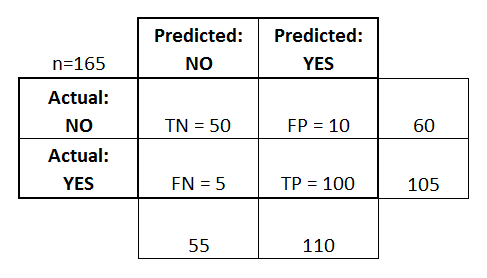
\includegraphics[width=0.5\textwidth]{confusion_matrix}
\caption{confusion matrix \protect\footnotemark{}}
\label{fig:confusion_matrix}
\end{figure}
\footnotetext{\url{https://docs.microsoft.com/en-us/azure/machine-learning/machine-learning-evaluate-model-performance}}


\subsubsection{Precision, Recall, F1 and UAC}
The \textbf{precision} of the classifier is the proportion of positives that are classified correctly: TP/(TP+FP). This is used for questions such as "Out of the pages that were classified as category A, how many were classified correctly?".\\

the \textbf{recall} of the classifier is used to answer the question "What percentage of the pages that fit category A were classified correctly?". In other words: TP/(TP+FN).\\

The \textbf{F1 Score} uses both precision and consideration. It is computed by using the following formula: F1 = 2 (precision x recall) / (precision + recall). The F1 score summarised evaluation in a single number, but for evaluation it is better to use recall and precision to understand the behaviour of the classifier. \\

The \textbf{Receiver Operating Characteristic (ROC) curve} and the corresponding \textbf{Area Under the Curve (AUC) value} can be used to inspect the true positive rate (Recall) vs. the false positive rate (FP / (FP + TN). To do this, the possibilities pages are correctly classified are needed. For each threshold on these probabilities for the classifier, the true positive rate and the false positive rate are calculated and are plotted in a graph, which results in something like \ref{fig:UAC}. The closer the ROC curve is to the upper left corner, the better the classifier's performance is. When close to the diagonal of the plot, the classifier tends to make predictions close to random guessing. The UAC value is the are under the ROC curve.

\begin{figure}[h]
\centering
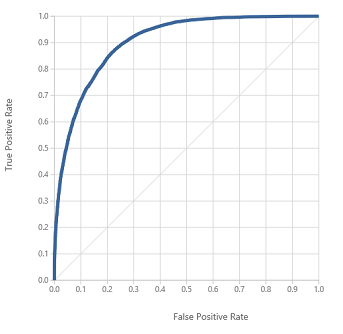
\includegraphics[width=0.5\textwidth]{UAC}
\caption{ROC / UAC graph \protect\footnotemark{}}
\label{fig:UAC}
\end{figure}
\footnotetext{\url{https://docs.microsoft.com/en-us/azure/machine-learning/machine-learning-evaluate-model-performance}}

\subsection{Evaluation of Relation Scores}
Evaluating relation scores is done differently. An important factor here is that cities have a natural relation due to their geographical position \cite{tobler1970computer}, so one would expect cities that lie close to each other are more related than cities that are on different sides of the country. This natural relation can be represented using the Gravity Model by Reilly \cite{reilly1931law}. The Gravity Model describes that the expected relation between two cities is based on the population of the two cities and the distance between these cities. A relation between two cities that is extracted from the data should thus expose a similar relative score as they would for the gravity model. Consider for example Amsterdam and Hoofddorp, which are cities that lie close to each other. Amsterdam is a large city, whereas Hoofddorp is much smaller. However, due to their close geographical position, the score that results from the Gravity Model would be high. If they turn out to have a very high score in our system, that would imply that the system is correct. Besides the Gravity Model, one can rely on the opinion of an expert in the field of urbanism that can judge whether an extracted relation is close to reality or not. We therefore agreed with the client that they would decide on a small set of relations whether they are correct. Lastly, the relations in the Randstad, a large urban area with the four largest cities of the Netherlands, have been examined before on the basis of firms \cite{van2010economic}. These relations can be compared to those extracted by the system.

\section{Fulfilment of Requirements}
In section \ref{sec:reqs} we declared the requirements for our program. Table \ref{requirements_pass/fail} shows which of these requirements passed or failed. \\
The program works as intended so all must haves passed. \\
There are however two should haves which failed. Finding correct relations proved more time-consuming than expected therefor our algorithm only discerns the top level relations (e.g. trade) and not sub levels (e.g. food trade). Furthermore there are a lot of places with duplicate names, yet no complete lists of these duplicates are available. Therefor it is less easy implementable than first thought. \\
Since other, more important, tasks took longer to implement than intended we did not make implement functionality to use Delpher to characterise relationships. We did add functionality to visualise the data by using a map. \\
As expected the would likes did not pass. It is theoretically possible to show all connections of all places on the map at the same time. However, it would result in a completely filled in map because there is a line for each relation so one would not be able to get any useful information from this.

\todo{more about not mentioned pass/fail, name reqs?}

\begin{table}[h]
\centering
\caption{Requirements pass fail}
\label{requirements_pass/fail}
\begin{tabular}{llllllll}
\begin{tabular}[c]{@{}l@{}}Must \\ Haves\end{tabular} & \begin{tabular}[c]{@{}l@{}}Pass /\\ Fail\end{tabular} & \begin{tabular}[c]{@{}l@{}}Should \\ haves\end{tabular} & \begin{tabular}[c]{@{}l@{}}Pass /\\ Fail\end{tabular} & \begin{tabular}[c]{@{}l@{}}Could \\ Haves\end{tabular} & \begin{tabular}[c]{@{}l@{}}Pass /\\ Fail\end{tabular} & \begin{tabular}[c]{@{}l@{}}Would\\ Haves\end{tabular} & \begin{tabular}[c]{@{}l@{}}Pass /\\ Fail\end{tabular} \\
1                                                     & Pass                                                  & 1                                                       & Fail                                                  & 1                                                      & Fail                                                  & 1                                                     & \todo{Pass?}                                                      \\
2                                                     & Pass                                                  & 2                                                       & Pass                                                  & 2                                                      & Pass                                                  & 2                                                     & Fail                                                       \\
3                                                     & Pass                                                  & 3                                                       & Pass                                                  &                                                        &                                                       & 3                                                     &                                                       \\
4                                                     & Pass                                                  & 4                                                       & Fail                                                  &                                                        &                                                       &                                                       &                                                       \\
5                                                     & Pass                                                  &                                                         &                                                       &                                                        &                                                       &                                                       &                                                      
\end{tabular}
\end{table}

\section{Process}

\subsection{Collaboration Between the Team Members}
The collaboration between the team members went well. The team members worked in a room in the faculty of architecture from 9-5 each day. Three of the four team members knew each other already. The work was divided even over the team members. 

\subsection{Collaboration Between the Team Members and the TU Delft Coach}
Each week 9:30 on Monday the team members had a meeting with the TU Delft coach. In the beginning there were some communication issues between the team and the coach but as the process went on communication became better.
\todo{Claudia absent twice}

\subsection{Collaboration Between the Team Members and the Client}
The collaboration between the team members and the client was good as well. 
Weekly meetings helped the team members making the product as good as possible to the clients wishes. 

\section{Ethics}
When using our program, there are two ethical issues that may arrive. The first is due to the fact that pages may be downloaded and stored, which may result in privacy or copyright issues. The second is about what the results of our program may be used for, and how the world will react to this.

\subsubsection{Storage}
One ethical issue is due to the storing of data. Since we store random web pages we do not know whether or not these pages may contain private or copyrighted data. For instance news articles could be downloaded and stored whilst this could violate the copyright issues. For most free news sites this is not a problem but this especially becomes a problem when using Delpher as a data source. Therefor if this source is added it must also be ensured that the data is stored in a safe way.

\subsubsection{Influence}
Another issue that may occur is the influence this kind of research may have. If there is indeed a correlation between the results of our program and the economic growth of cities this may influence the behaviour of investors, companies and cities. Investors may look at the data and decide to invest in companies from more growing cities. Companies may use this data to decide where to build their new offices. And cities may change their policies based on the results. In future executions of our system it may also occur that data is being manipulated. Involved parties which put extra data online containing the names of cities they want to have a better result for. Whilst these issues may occur, we do not suspect our system to have a large enough impact to cause this. It may rather be a step towards these effects. Over time the effects will become clearer and they should be taken into account when continuing research in this field.
